% !TeX root = main.tex
% !TEX program = pdflatex

% =============================================================
% CAPÍTULO 10 — ESQUELETO (pendiente de redactar)
% Mapea con el descriptor oficial: "Sensores industriales" (contenido
% suelto en el descriptor, sin capítulo propio -- se aloja aquí junto al
% lazo 4-20mA/HART) + RA9 (Configurar un sensor inteligente industrial,
% modificando sus parámetros con software especializado).
% Al ser un curso de Telecomunicaciones, priorizar los buses de campo
% relevantes en instrumentación de laboratorio/RF-óptica sobre la
% automatización puramente fabril.
% =============================================================

\chapter{Sensores Industriales, Sensores Inteligentes y Buses Digitales}\label{cap:buses}

A lo largo de los Capítulos~\ref{cap:resistivos} a~\ref{cap:opticos} hemos elegido el sensor adecuado y acondicionado su señal con amplificadores y filtros de precisión; el Capítulo~\ref{cap:daq} la convirtió en un número y el Capítulo~\ref{cap:ruido} nos enseñó a defenderla del ruido y de las interferencias del entorno. En todo ese recorrido ha estado presente una suposición que hasta ahora no habíamos puesto en duda: que el sensor y su electrónica de adquisición están a pocos centímetros de distancia, sobre la misma placa o el mismo banco de laboratorio. Basta trasladar la medida a una planta industrial --o a un montaje de laboratorio real, con la cámara climática, el electroimán o la antena de medida a decenas de metros del puesto de control-- para que esa suposición se rompa: la señal acondicionada debe recorrer un cable largo y, con él, se agravan a la vez los dos problemas que ya conocemos. La resistencia del propio cable, que en la conexión a 2 hilos se sumaba a la del sensor (Sección~\ref{sec:conexion_hilos}), deja de ser una fracción de ohmio para volverse del orden de la variación que produce el propio mensurando, y además deriva con la temperatura del tendido; y las interferencias acopladas (Sección~\ref{sec:acoplamientos}) crecen con la longitud de ese cableado, porque un par de hilos largo es a la vez una antena y un bucle de tierra mucho más eficaces que una pista de circuito impreso.

La instrumentación industrial resolvió este problema hace décadas con una idea que sigue plenamente vigente: transmitir la información como \emph{corriente} en lugar de como tensión, en el lazo \SI{4}{\milli\ampere} a \SI{20}{\milli\ampere} que se estudia en la Sección~\ref{sec:lazo_420} y sobre el que el protocolo HART (Sección~\ref{sec:hart}) superpone después un canal digital con el que configurar y consultar el instrumento sin interrumpir la medida. Dentro del propio equipo, y a distancias cortas, ese mismo papel lo cumplen los buses I2C y SPI (Sección~\ref{sec:i2c_spi}), que son de hecho la salida que ofrecen hoy la mayoría de los sensores MEMS; y cuando acondicionamiento, conversión y microcontrolador se integran en un mismo encapsulado nace el \emph{sensor inteligente} (Sección~\ref{sec:smart_sensors}), capaz de anunciar sus propias unidades, rango y calibración y de ser reconfigurado por software. Este capítulo recorre, por tanto, el último tramo de la cadena de medida --del acondicionador al sistema de adquisición, y del dato analógico al dato digital-- en el entorno, industrial o de laboratorio, donde la distancia y el ruido obligan a abandonar la transmisión en tensión~\cite{pallasareny2000sensors,bentley2004measurement}.

\section{El Lazo de Corriente 4-20 mA}\label{sec:lazo_420}

La forma más directa de llevar una señal ya acondicionada hasta el sistema de adquisición es transmitirla como una tensión. Mientras el recorrido se mide en centímetros --el caso de todos los capítulos anteriores--, la diferencia entre la tensión que sale del acondicionador y la que llega al receptor es despreciable; pero en cuanto el sensor se aleja, como ocurre en una planta industrial o en un montaje de laboratorio con el instrumento en la cámara y el puesto de control a decenas de metros, el cableado y las interferencias que este recoge a lo largo del tendido se suman o se restan a la señal. La instrumentación de proceso resolvió ese problema hace décadas transmitiendo la información como \emph{corriente} en lugar de como tensión, y lo hizo con un rango normalizado que sigue plenamente vigente: la norma \emph{IEC 60381-1} fija la señal de corriente continua de \SI{4}{\milli\ampere} a \SI{20}{\milli\ampere} para el intercambio de información entre los elementos de un sistema de control de proceso~\cite{iec60381_1_1982}. En esta sección veremos por qué la corriente es inmune a la resistencia del cable, cómo se alimenta y se lee el lazo, por qué su cero está en \SI{4}{\milli\ampere} y qué limitaciones impone ese formato, que son justamente las que justifican el canal digital de la Sección~\ref{sec:hart}.

\subsection{¿Por Qué Corriente y No Tensión?}\label{sub:por_que_corriente}

En una transmisión en tensión, el transmisor se comporta como una fuente de tensión con una impedancia de salida $R_{out}$ y el receptor como un voltímetro de impedancia de entrada $R_{in}$, unidos ambos por un par de hilos que aportan una resistencia $R_w$ cada uno. La tensión que llega al receptor es entonces
\begin{equation}\label{eq:error_cable_tension}
    v_{rx} = v_{tx}\,\frac{R_{in}}{R_{in} + 2R_w + R_{out}} \approx v_{tx}\left(1 - \frac{2R_w}{R_{in}}\right)
\end{equation}
donde la aproximación es válida cuando $R_w \ll R_{in}$. El error es sistemático, proporcional a la longitud del tendido y sensible a su temperatura --el cobre aumenta su resistividad un \SI{0.4}{\percent} por cada grado centígrado--, esto es, el mismo efecto de carga que ya nos obligó a pasar de 2 a 3 y 4 hilos en la medida de resistencias (Sección~\ref{sec:conexion_hilos}). Y existe un segundo inconveniente que no depende de la relación de impedancias: toda tensión inducida \emph{en serie} con el lazo --un acoplamiento inductivo con un conductor de potencia próximo (Sección~\ref{sub:acoplamiento_inductivo}) o una diferencia de potencial entre las tierras de los dos extremos (Sección~\ref{sec:tierras})-- se suma directamente a la señal recibida, porque un receptor de alta impedancia no atenúa en absoluto esa perturbación.

El lazo de corriente invierte los papeles de ambos extremos. El transmisor es ahora una fuente de corriente \emph{regulada}, cuya impedancia de salida es altísima --del orden de megaohmios: esa es precisamente la forma en que regula--, y el receptor un amperímetro de baja impedancia, materializado en la práctica mediante una resistencia de carga o \emph{shunt} $R_s$ sobre la que se mide la caída de tensión. Como por todo el lazo circula la misma corriente, la resistencia del cableado desaparece de la relación entre la variable transmitida y la recibida: ni una longitud mayor, ni un terminal oxidado, ni un tendido más caliente modifican $I$, siempre que la fuente conserve margen de tensión para seguir forzándola (Sección~\ref{sub:presupuesto_lazo}). Y frente a una perturbación $e_n$ inducida en serie, la corriente de ruido que esta inyecta en el lazo es
\begin{equation}\label{eq:ruido_serie_lazo}
    i_n = \frac{e_n}{R_{out} + 2R_w + R_s} \approx \frac{e_n}{R_{out}}
\end{equation}
es decir, la misma perturbación que en tensión se sumaba íntegra a la señal queda aquí dividida por la elevadísima impedancia de salida del transmisor. Es exactamente el argumento físico que ya aprovechamos al alimentar el puente de Wheatstone con corriente (Sección~\ref{sec:puente_wheatstone}): forzar la corriente hace que la medida dependa de la magnitud del sensor y no de las resistencias parásitas del camino, solo que ahora esa resistencia parásita es un tendido de cientos de metros. La Figura~\ref{fig:error_cable} cuantifica el error que ese tendido introduce en cada uno de los dos modos de transmisión.

\begin{marginfigure}
    \centering
    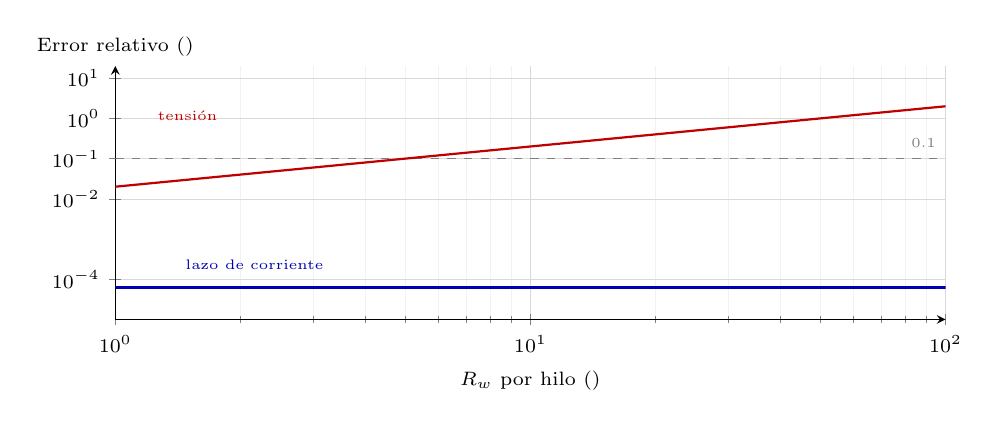
\begin{tikzpicture}
        \begin{axis}[
            width=\linewidth, height=4.8cm,
            xlabel={$R_w$ por hilo (\si{\ohm})},
            ylabel={Error relativo (\si{\percent})},
            xmode=log, ymode=log,
            xmin=1, xmax=100, ymin=1e-5, ymax=2e1,
            axis lines=left,
            grid=both,
            grid style={line width=.1pt, draw=gray!10},
            major grid style={line width=.2pt,draw=gray!30},
            font=\scriptsize,
            xtick={1,10,100},
            ytick={1e-4,1e-2,1e-1,1,1e1},
            every axis y label/.style={at=(current axis.above origin), anchor=south},
        ]
            % Error del lazo de corriente: solo la perturbación en serie / Rout
            \addplot[thick, blue!70!black, domain=1:100, samples=2] {6.25e-5};
            \node[blue!70!black, font=\tiny, anchor=south west] at (axis cs:1.4,1e-4) {lazo de corriente};
            % Precisión típica de un instrumento
            \draw[dashed, gray] (axis cs:1,1e-1) -- (axis cs:100,1e-1);
            \node[gray, font=\tiny, anchor=south east] at (axis cs:100,1.1e-1) {\SI{0.1}{\percent}};
            % Error de la transmisión en tensión: 2Rw/Rin con Rin = 10 kohm
            \addplot[thick, red!75!black, domain=1:100, samples=2] {x/50};
            \node[red!75!black, font=\tiny, anchor=south west] at (axis cs:1.2,0.5) {tensión};
        \end{axis}
    \end{tikzpicture}
    \caption[Error por resistencia del cable: tensión frente a lazo de corriente.]{Error relativo introducido por la resistencia del cableado, en escala logarítmica, en función de la resistencia por hilo $R_w$: para una transmisión en tensión con entrada de \SI{10}{\kilo\ohm} (ecuación~\eqref{eq:error_cable_tension}) y para el lazo de corriente, evaluado este para una perturbación inducida en serie de \SI{10}{\milli\volt} y una impedancia de salida del transmisor de \SI{1}{\mega\ohm} (ecuación~\eqref{eq:ruido_serie_lazo}). El error de la transmisión en tensión crece con la longitud del tendido y alcanza la precisión típica de un instrumento (\SI{0.1}{\percent}, línea discontinua) con apenas \SI{5}{\ohm} por hilo, es decir, unos \SI{70}{\meter} de par de \SI{0.5}{\milli\meter\squared}; el del lazo de corriente queda tres órdenes de magnitud por debajo y no depende de $R_w$ mientras la fuente conserve margen de tensión (Sección~\ref{sub:presupuesto_lazo}).}\label{fig:error_cable}
\end{marginfigure}

A las dos ventajas anteriores se añade una tercera, de carácter práctico: como la corriente entra y sale por el mismo par de hilos, la tensión de modo común --la diferencia de potencial entre dos tierras separadas por decenas de metros, que en un entorno industrial puede alcanzar varios voltios-- no se suma a la señal, porque el receptor mide únicamente la corriente que atraviesa el par. Al retorcer los dos conductores (par trenzado), las corrientes, iguales y opuestas, cancelan además el campo magnético que generan, de modo que el lazo apenas emite y apenas capta por vía inductiva; es el mismo razonamiento que justifica el par trenzado en el filtrado de modo común (Sección~\ref{sec:filtrado_emi}). La Tabla~\ref{tab:tension_vs_corriente} resume la comparación entre ambos modos de transmisión.

\begin{table}[ht]
    \centering
    \small
    \setlength{\tabcolsep}{3pt}
    \begin{tabularx}{\linewidth}{@{} >{\raggedright\arraybackslash}p{0.24\linewidth} >{\centering\arraybackslash}X >{\centering\arraybackslash}X @{}}
        \toprule
        \textbf{Aspecto} & \textbf{Señal en tensión} & \textbf{Lazo 4-20 mA} \\
        \midrule
        Magnitud medida en el receptor & Tensión, con entrada de $R_{in}$ alta & Corriente, sobre un \emph{shunt} $R_s$ \\
        Resistencia del cable $R_w$ & Error $\propto 2R_w/R_{in}$, crece con la longitud y la temperatura & Nulo: la corriente está regulada \\
        Perturbación inducida en serie & Se suma íntegra a la señal & Dividida por $R_{out}$ (ec.~\eqref{eq:ruido_serie_lazo}) \\
        Tensión de modo común & Debe rechazarla la etapa de entrada (CMRR) & No interviene: el par es diferencial \\
        Fallo del cable o del sensor & Indistinguible de una medida de 0 \% (cero muerto) & Inmediato: solo el lazo abierto da 0 mA (cero vivo) \\
        Alimentación del transmisor & Hilos de alimentación adicionales & La suministra el propio par (2 hilos) \\
        Distancia típica & Metros, dentro del equipo & Hasta \SI{2}{\kilo\meter} \\
        \bottomrule
    \end{tabularx}
    \caption[Transmisión en tensión frente a lazo de corriente 4-20 mA.]{Comparación entre la transmisión de una señal acondicionada como tensión y como corriente. La ventaja del lazo no reside en la electrónica del transmisor, sino en que la magnitud transmitida no depende de la resistencia del camino: ni la caída de tensión en el cable (ecuación~\eqref{eq:error_cable_tension}) ni las tensiones inducidas en serie (ecuación~\eqref{eq:ruido_serie_lazo}) alteran una corriente que la fuente mantiene regulada.\protect\label{tab:tension_vs_corriente}}
\end{table}

\marginnote{\textbf{La clave física:} el lazo no elimina la resistencia del cable ni las perturbaciones inducidas, sino que las hace irrelevantes al regular la corriente: mientras la fuente pueda forzar los \SI{20}{\milli\ampere}, el receptor recibe la misma corriente que generó el transmisor, con independencia de lo que ocurra en el camino.}

\subsection{El Cero Vivo: Por Qué el Cero Está en 4 mA}\label{sub:cero_vivo}

Fijado el principio físico, la elección del rango no es arbitraria: la señal podía haberse normalizado de 0 a 20 mA y, sin embargo, el estándar optó por \SI{4}{\milli\ampere} a \SI{20}{\milli\ampere}. Con la variable medida expresada como porcentaje del rango, la correspondencia entre magnitud y corriente es lineal,
\begin{equation}\label{eq:recta_420}
    I = \SI{4}{\milli\ampere} + \SI{16}{\milli\ampere}\cdot\frac{m - m_{min}}{m_{max} - m_{min}}
\end{equation}
de modo que a cada punto porcentual del rango le corresponden \SI{0.16}{\milli\ampere}.

La razón de desplazar el cero --el llamado \emph{cero vivo}, \textit{live zero}, frente al \emph{cero muerto} del rango 0-20 mA-- es que \SI{0}{\milli\ampere} es precisamente lo que el lazo presenta por sí solo cuando no hay información que transmitir: un cable cortado, un transmisor sin alimentación o un sensor averiado dejan el lazo en circuito abierto y el receptor lee cero. Con un cero muerto, esa lectura sería indistinguible de una medida legítima del 0 \% del rango --un depósito vacío, una temperatura de \SI{0}{\celsius}-- y el operador no tendría forma de saber si el proceso está en su mínimo o el instrumento ha dejado de funcionar. Desplazando el cero a \SI{4}{\milli\ampere}, toda la banda inferior a ese valor queda libre para señalar un fallo, de manera que cualquier lectura por debajo de \SI{4}{\milli\ampere} es, sin ambigüedad, una avería.

Hay además una razón de tipo energético que empuja el límite hacia arriba: un transmisor de 2 hilos se alimenta del propio lazo (Sección~\ref{sub:presupuesto_lazo}), de modo que su electrónica consume una corriente de reposo que no puede dedicar a la señal; si el 0 \% correspondiera a \SI{0}{\milli\ampere}, el instrumento carecería de energía precisamente en el extremo inferior del rango. Por eso la recomendación \emph{NAMUR NE 43} fija la banda de medida válida entre \SI{3.8}{\milli\ampere} y \SI{20.5}{\milli\ampere} y reserva los valores inferiores a \SI{3.6}{\milli\ampere} y superiores a \SI{21}{\milli\ampere} para la señalización de fallo, con sendas bandas de guarda que permiten distinguir una avería de una medida saturada~\cite{namur_ne43_1994}. La Figura~\ref{fig:zonas_420} representa esa zonificación sobre la recta de transferencia.

\begin{marginfigure}
    \centering
    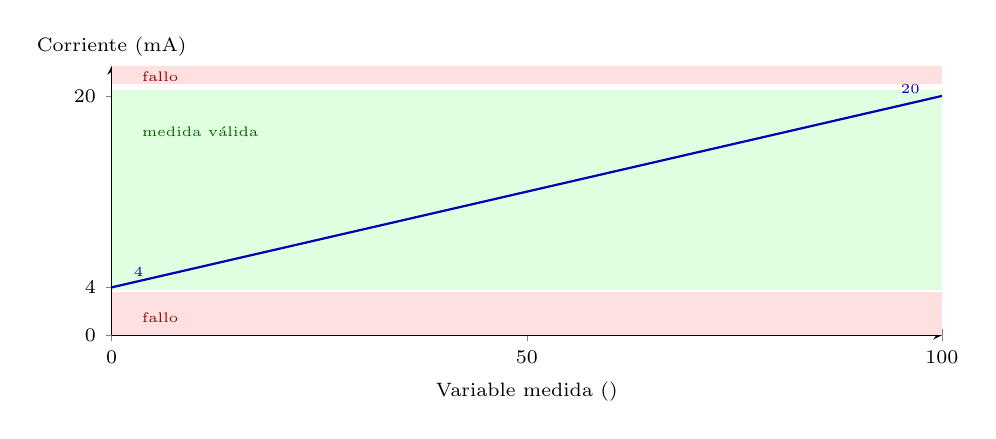
\begin{tikzpicture}
        \begin{axis}[
            width=\linewidth, height=5cm,
            xlabel={Variable medida (\si{\percent})},
            ylabel={Corriente (mA)},
            xmin=0, xmax=100, ymin=0, ymax=22.5,
            axis lines=left,
            font=\scriptsize,
            xtick={0,50,100},
            ytick={0,4,20},
            every axis y label/.style={at=(current axis.above origin), anchor=south},
        ]
            % Zonas de señal (NAMUR NE 43)
            \fill[red!12] (axis cs:0,0) rectangle (axis cs:100,3.6);
            \fill[green!12] (axis cs:0,3.8) rectangle (axis cs:100,20.5);
            \fill[red!12] (axis cs:0,21) rectangle (axis cs:100,22.5);
            % Recta de transferencia
            \addplot[thick, blue!70!black, domain=0:100, samples=2] {4 + 0.16*x};
            % Etiquetas de las zonas
            \node[red!60!black, font=\tiny, anchor=west] at (axis cs:2.5,1.5) {fallo};
            \node[green!40!black, font=\tiny, anchor=west] at (axis cs:2.5,17) {medida válida};
            \node[red!60!black, font=\tiny, anchor=west] at (axis cs:2.5,21.6) {fallo};
            % Extremos de la recta
            \node[blue!70!black, font=\tiny, anchor=south west] at (axis cs:1.5,4.1) {\SI{4}{\milli\ampere}};
            \node[blue!70!black, font=\tiny, anchor=south east] at (axis cs:98.5,19.4) {\SI{20}{\milli\ampere}};
        \end{axis}
    \end{tikzpicture}
    \caption[Zonas de señal del lazo 4-20 mA según NAMUR NE 43.]{Zonas de señal del lazo de corriente y recta de transferencia entre la variable medida y la corriente (ecuación~\eqref{eq:recta_420}). El cero vivo hace que el 0 \% de la medida se transmita con \SI{4}{\milli\ampere}, de modo que la banda inferior a \SI{3.6}{\milli\ampere} --y la superior a \SI{21}{\milli\ampere}-- quedan disponibles para señalar un fallo del instrumento, sin confundirse con una medida válida. Las bandas de guarda (\SI{3.6}{\milli\ampere} a \SI{3.8}{\milli\ampere} y \SI{20.5}{\milli\ampere} a \SI{21}{\milli\ampere}) separan la medida saturada de la avería.}\label{fig:zonas_420}
\end{marginfigure}

\marginnote{\textbf{Regla mnemotécnica:} los 16 mA de recorrido cubren el 100 \% del rango de medida, es decir, \SI{0.16}{\milli\ampere} por cada punto porcentual; y un lazo cortado se lee siempre como \SI{0}{\milli\ampere}, por debajo de cualquier medida válida.}

\subsection{Presupuesto de Tensión del Lazo}\label{sub:presupuesto_lazo}

Como se representa en la Figura~\ref{fig:lazo_420}, el lazo es un circuito serie alimentado por una fuente de continua --habitualmente \SI{24}{\volt}-- que debe forzar la corriente a través de la resistencia total del camino: los dos hilos del tendido, la resistencia de carga del receptor y, en su caso, las protecciones de entrada. Como el transmisor necesita un mínimo de tensión para funcionar, el lazo se comprueba con la condición
\begin{equation}\label{eq:presupuesto_lazo}
    V_{alim} \ge I\left(2R_w + R_s\right) + V_{tx,min}
\end{equation}
que, evaluada en el peor caso ($I = \SI{20}{\milli\ampere}$), fija la resistencia máxima que admite el lazo:
\begin{equation}\label{eq:r_lazo_max}
    R_{lazo,max} = \frac{V_{alim} - V_{tx,min}}{\SI{20}{\milli\ampere}}
\end{equation}
Nótese que la fuente no avisa: si se supera ese límite, el transmisor se queda sin margen de tensión, deja de poder regular la corriente y la lectura cae hacia cero, confundiéndose con un fallo. Se trata, por tanto, de un cálculo de diseño y no de algo que convenga descubrir durante la puesta en marcha.

\begin{marginfigure}
    \centering
    \shorthandoff{>}
    \begin{tikzpicture}[american, scale=0.85]
        % --- Fuente de alimentación y transmisor (rama izquierda) ---
        \draw (0,0.5) to[battery1, l_=$V_{alim}$] (0,1.7);
        \draw[thick] (-0.85,1.7) rectangle (0.85,3.3);
        \node[font=\scriptsize, align=center] at (0,2.8) {Transmisor};
        \node[font=\scriptsize, align=center] at (0,2.3) {(2 hilos)};
        \draw[<-] (-1.7,2.5) -- (-0.85,2.5) node[midway, above, font=\scriptsize] {$m$};
        % --- Hilo superior con su resistencia ---
        \draw (0,3.3) -- (0,4.2) to[R, l=$R_w$] (2.4,4.2) -- (3.8,4.2) node[circ]{};
        % --- Rama derecha: receptor (shunt) ---
        \draw (3.8,4.2) to[R, l=$R_s$] (3.8,0.5) node[circ]{};
        % --- Hilo inferior con su resistencia y retorno ---
        \draw (3.8,0.5) to[R, l=$R_w$] (1.4,0.5) -- (0,0.5);
        % --- Voltímetro del receptor, en paralelo con Rs ---
        \draw (3.8,4.2) -- (5.1,4.2) to[voltmeter] (5.1,0.5) -- (3.8,0.5);
        \node[font=\scriptsize, align=center] at (4.45,-0.5) {Sistema de\\adquisición};
        % --- Sentido de la corriente ---
        \draw[->, red!75!black, thick] (2.7,4.45) -- (3.5,4.45)
            node[midway, above, font=\scriptsize, black] {$I$};
    \end{tikzpicture}
    \caption[Lazo de corriente 4-20 mA con transmisor de dos hilos.]{Lazo de corriente con un transmisor de 2 hilos alimentado por el propio lazo. La fuente de \SI{24}{\volt} suministra la corriente que la electrónica del transmisor regula entre \SI{4}{\milli\ampere} y \SI{20}{\milli\ampere} en función del mensurando $m$; esa misma corriente atraviesa las resistencias $R_w$ de los dos hilos y la resistencia de carga $R_s$ del receptor, donde se mide como una tensión $I \cdot R_s$.}\label{fig:lazo_420}
\end{marginfigure}

\marginnote{\textbf{Ejemplo:} un lazo alimentado a 24 V con un transmisor que exige 12 V admite hasta \SI{600}{\ohm} (ecuación~\eqref{eq:r_lazo_max}). Un tendido de ida y vuelta de \SI{2}{\kilo\meter} sobre par trenzado de \SI{0.5}{\milli\meter\squared} aporta $2 \cdot \SI{2000}{\meter} \cdot \SI{0.035}{\ohm\per\meter} \approx \SI{140}{\ohm}$ que, junto a los \SI{250}{\ohm} del receptor, suman \SI{390}{\ohm}: dentro del presupuesto, y al transmisor le restan $24 - 0.02 \cdot 390 = \SI{16.2}{\volt}$.}

La elección de $R_s$ no es casual. Con \SI{250}{\ohm}, la corriente del lazo se traduce en una tensión de \SI{1}{\volt} a \SI{5}{\volt}, que es el interfaz clásico de las entradas de adquisición: el cero vivo se convierte así en un desplazamiento del 20 \% del fondo de escala, y la banda de fallo ($\le \SI{3.6}{\milli\ampere}$) cae por debajo de \SI{0.9}{\volt}, es decir, dentro de ese 20 \% que el cero vivo ha liberado. El convertidor puede distinguir entonces, sin circuitería adicional, una medida válida de un fallo del instrumento (Capítulo~\ref{cap:daq}).

\subsection{Limitaciones del Lazo Analógico}\label{sub:limitaciones_lazo}

Con lo visto hasta aquí, el lazo de corriente es un canal extraordinariamente robusto, normalizado y barato por punto de medida --dos hilos que alimentan y transmiten a la vez--, y además su degradación es predecible: una conexión deficiente produce una lectura de fallo, nunca un dato corrupto. Su limitación no está, por tanto, en la robustez, sino en la cantidad de información que transporta: un único valor analógico. El receptor no puede saber qué instrumento tiene conectado, en qué unidades mide, cuándo se calibró por última vez ni qué diagnósticos internos ha registrado el transmisor; y si un mismo equipo mide dos variables --por ejemplo, la temperatura y la presión de una cámara--, cada una exige su propio par de hilos y su propia entrada de adquisición. A esto se añade que la configuración del instrumento (su rango, su amortiguación, su unidad) es local: hay que actuar sobre el propio transmisor, con un configurador manual conectado al lazo o abriendo su envolvente en campo.

Esa carencia de información es la que resuelve superponer un canal digital al mismo par de hilos, que es la idea del protocolo HART (Sección~\ref{sec:hart}): la corriente sigue siendo la medida continua y rápida, mientras que el canal digital transporta la identificación, la calibración y los parámetros de configuración. Es el primer paso hacia el instrumento inteligente (Sección~\ref{sec:smart_sensors}) y el elemento que permite ajustar un sensor industrial por software desde el puesto de control, sin necesidad de acceder físicamente a él.

\section{El Protocolo HART}\label{sec:hart}

Para el sistema de control, la información que llega por un lazo de corriente es un único número. La sección anterior ha mostrado que ese número es notablemente fiel, pero nada dice de qué instrumento procede, en qué unidades está, cuándo se calibró por última vez ni si su electrónica ha registrado alguna anomalía. La respuesta que adoptó la instrumentación de proceso --y que todavía hoy domina-- no fue sustituir el lazo, sino aprovecharlo: el protocolo \emph{HART} (\textit{Highway Addressable Remote Transducer}), desarrollado por Rosemount a mediados de los años ochenta, publicado como estándar abierto en 1986 y mantenido hoy por FieldComm Group como norma \emph{IEC 61158 Type 20}, superpone un canal digital a la misma señal de \SI{4}{\milli\ampere} a \SI{20}{\milli\ampere}~\cite{hart_spec_2020}. El resultado es una convivencia que explica su éxito: el sistema de control heredado sigue leyendo la corriente analógica sin modificar ni un cable, mientras un maestro digital dialoga con el instrumento por el mismo par. En esta sección veremos cómo consiguen coexistir ambas señales, en qué configuraciones se puede explotar el canal digital y qué información añade.

\subsection{El Canal Digital sobre el Lazo}\label{sub:canal_hart}

El requisito de partida es que ningún canal interfiera con el otro, y la clave para lograrlo es la separación de sus bandas de frecuencia. La medida analógica es una señal lenta --continua o cuasiestática, con contenido espectral que no pasa de unos pocos hercios--, de modo que el canal digital puede situarse muy por encima de ella. HART emplea una modulación por desplazamiento de frecuencia (\textsc{frequency shift keying, fsk}) con dos tonos bien alejados de la banda de la medida: \SI{1200}{\hertz} para el bit 1 y \SI{2200}{\hertz} para el bit 0, a una velocidad fija de \SI{1200}{\bit\per\second}. La corriente que circula por el lazo es, por tanto, la suma de las dos señales,
\begin{equation}\label{eq:hart_fsk}
    i(t) = \underbrace{I_{DC}(m)}_{\text{medida analógica}} \;+\; \underbrace{I_0 \sin\!\left(2\pi f_k t\right)}_{\text{canal digital}}, \qquad f_k \in \left\{\SI{1200}{\hertz}, \SI{2200}{\hertz}\right\}
\end{equation}
con una amplitud de los tonos de $I_0 = \SI{0.5}{\milli\ampere}$ ($\pm$ \SI{0.5}{\milli\ampere} alrededor del valor de continua). Como el valor medio de la componente alterna es nulo, la corriente de medida no se desplaza: el canal digital viaja sin falsear la medida analógica. La Figura~\ref{fig:hart_fsk} representa ambas componentes en el tiempo y su separación en frecuencia.

\begin{marginfigure}
    \centering
    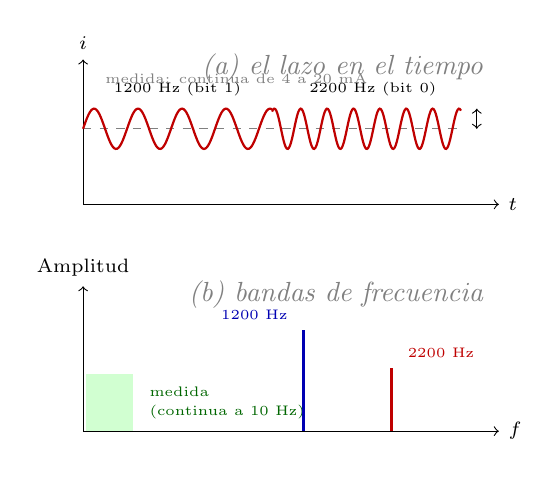
\begin{tikzpicture}[scale=0.8]
        % ── (a) el lazo en el tiempo ──────────────────────────
        \begin{scope}
            \draw[->] (0,0) -- (6.6,0) node[right, font=\scriptsize] {$t$};
            \draw[->] (0,0) -- (0,2.3) node[above, font=\scriptsize] {$i$};
            \draw[gray, dashed] (0,1.2) -- (6.0,1.2);
            \draw[red!75!black, thick] plot[domain=0:3.0, samples=140] (\x,{1.2+0.32*sin(deg(9*\x))});
            \draw[red!75!black, thick] plot[domain=3.0:6.0, samples=180] (\x,{1.2+0.32*sin(deg(15*\x))});
            \draw[<->, thin] (6.25,1.2) -- (6.25,1.52);
            \node[font=\tiny, anchor=south] at (1.5,1.56) {1200 Hz (bit 1)};
            \node[font=\tiny, anchor=south] at (4.6,1.56) {2200 Hz (bit 0)};
            \node[gray, font=\tiny, anchor=west] at (0.2,2.0) {medida: continua de 4 a 20 mA};
            \node[anchor=north east, font=\itshape, gray] at (6.5,2.55) {(a) el lazo en el tiempo};
        \end{scope}
        % ── (b) bandas de frecuencia ──────────────────────────
        \begin{scope}[yshift=-3.6cm]
            \draw[->] (0,0) -- (6.6,0) node[right, font=\scriptsize] {$f$};
            \draw[->] (0,0) -- (0,2.3) node[above, font=\scriptsize] {Amplitud};
            \fill[green!18] (0.05,0) rectangle (0.8,0.9);
            \node[green!40!black, font=\tiny, anchor=west] at (0.9,0.62) {medida};
            \node[green!40!black, font=\tiny, anchor=west] at (0.9,0.3) {(continua a 10 Hz)};
            \draw[blue!70!black, very thick] (3.5,0) -- (3.5,1.6);
            \node[blue!70!black, font=\tiny, anchor=south east] at (3.4,1.62) {1200 Hz};
            \draw[red!75!black, very thick] (4.9,0) -- (4.9,1.0);
            \node[red!75!black, font=\tiny, anchor=south west] at (5.0,1.02) {2200 Hz};
            \node[anchor=north east, font=\itshape, gray] at (6.5,2.55) {(b) bandas de frecuencia};
        \end{scope}
    \end{tikzpicture}
    \caption[Señal HART: canal digital FSK superpuesto a la medida analógica.]{Separación de bandas del protocolo HART. \emph{(a)}~En el dominio del tiempo, la corriente del lazo es la medida analógica --una continua lenta, línea discontinua-- más los tonos del canal digital, cuya amplitud es de $\pm$\,\SI{0.5}{\milli\ampere} (flecha). Como el valor medio de los tonos es nulo, la lectura analógica no se altera. \emph{(b)}~En el dominio de la frecuencia, ambos canales ocupan bandas bien separadas: la medida ocupa desde continua hasta unos \SI{10}{\hertz}, mientras que los tonos FSK se sitúan en \SI{1200}{\hertz} y \SI{2200}{\hertz}. Esa separación es la que permite filtrar cada canal por separado --paso bajo en el receptor analógico, paso alto en el módem-- y que los tonos no aparezcan como ruido en la medida. El eje de frecuencias es esquemático, no lineal.}\label{fig:hart_fsk}
\end{marginfigure}

La separación de bandas hace posible la convivencia, pero no la hace gratuita. Superpuestos a la continua, los tonos de la ecuación~\eqref{eq:hart_fsk} oscilan la corriente del lazo \SI{1}{\milli\ampere} de pico a pico, algo más del \SI{6}{\percent} del recorrido de \SI{16}{\milli\ampere}: en la resistencia de carga del receptor --los \SI{250}{\ohm} del ejemplo de la Sección~\ref{sub:presupuesto_lazo}-- esas oscilaciones equivalen a una tensión de \SI{250}{\milli\volt} de pico a pico, un \SI{6}{\percent} del fondo de escala de la entrada, mucho más que la precisión de cualquier instrumento. Por eso la convivencia exige filtrar: la entrada analógica limita su ancho de banda a unos pocos hercios y descarta así los tonos, mientras que el módem HART interpone un filtro paso alto que ignora la componente continua y solo escucha su banda. El mismo razonamiento explica el mínimo de carga que exige el protocolo: el lazo debe presentar al menos \SI{250}{\ohm} para que los tonos generen una tensión detectable, y no conviene subir de unos \SI{1100}{\ohm}, que es el límite que impone el presupuesto de tensión de la Sección~\ref{sub:presupuesto_lazo}.

Las consecuencias de la velocidad son igual de importantes que las de la convivencia. A \SI{1200}{\bit\per\second}, y con once bits por carácter, el canal digital transporta del orden de cien caracteres por segundo: un intercambio de orden y respuesta tarda decenas o cientos de milisegundos. Es tiempo de sobra para leer una identificación, lanzar un diagnóstico o cambiar un rango, pero no para gobernar un lazo de control, que sigue confiando en la vía analógica.

\subsection{Modos de Operación}\label{sub:modos_hart}

HART es un protocolo maestro-esclavo y semidúplex: en cada momento habla un solo participante y el diálogo lo inicia siempre un maestro. Admite, sin embargo, \emph{dos} maestros, y esa sutileza resulta muy práctica: el sistema de control actúa como maestro primario y el técnico puede conectar su comunicador portátil como maestro secundario sobre el mismo lazo, de modo que consulta y configura el instrumento sin interrumpir la medida que el sistema de control sigue leyendo. La Figura~\ref{fig:modos_hart} esquematiza las dos configuraciones posibles y la Tabla~\ref{tab:modos_hart} las compara.

\begin{table}[ht]
    \centering
    \small
    \setlength{\tabcolsep}{3pt}
    \begin{tabularx}{\linewidth}{@{} >{\centering\arraybackslash}p{0.2\linewidth} >{\centering\arraybackslash}X >{\centering\arraybackslash}X @{}}
        \toprule
        \textbf{Aspecto} & \textbf{Punto a punto} & \textbf{Multidrop} \\
        \midrule
        Instrumentos por par & Uno (dirección 0) & Hasta 15 (direcciones 1 a 15) \\
        Corriente del lazo & La de la medida, de 4 a 20 mA & Fija en \SI{4}{\milli\ampere}: solo alimenta al instrumento \\
        Variable principal & Analógica y digital a la vez & Solo digital \\
        Velocidad de actualización & La de la vía analógica (milisegundos) & Dos o tres intercambios por segundo en todo el grupo \\
        Cableado & El de la instrumentación existente & Un único par para todo el grupo \\
        Uso típico & Lazos de control y medida en continuo & Monitorización lenta y diagnóstico de una batería de instrumentos \\
        Compatibilidad & Total con el 4-20 mA previamente instalado & Exige maestro HART y una dirección distinta por instrumento \\
        \bottomrule
    \end{tabularx}
    \caption[Modos de operación de HART: punto a punto frente a multidrop.]{Comparación de los dos modos de operación de HART. El modo punto a punto conserva intacta la vía analógica y añade información por el canal digital; el modo multidrop concentra varios instrumentos en un solo par a costa de renunciar a la medida analógica y de repartir una velocidad de comunicación de \SI{1200}{\bit\per\second} entre todos ellos.\protect\label{tab:modos_hart}}
\end{table}

\begin{marginfigure}
    \centering
    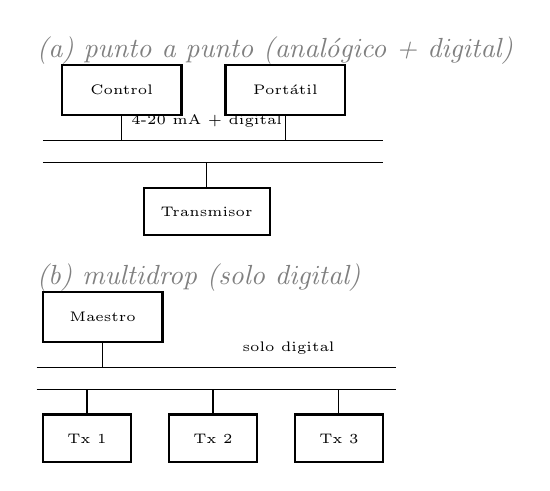
\begin{tikzpicture}[scale=0.8]
        % ── (a) punto a punto ────────────────────────────────
        \begin{scope}
            \node[anchor=north west, font=\itshape, gray] at (0.05,3.3) {(a) punto a punto (analógico + digital)};
            \draw[thick] (0.6,1.9) rectangle (2.5,2.7);
            \node[font=\tiny] at (1.55,2.3) {Control};
            \draw[thick] (3.2,1.9) rectangle (5.1,2.7);
            \node[font=\tiny] at (4.15,2.3) {Portátil};
            \draw (1.55,1.9) -- (1.55,1.5);
            \draw (4.15,1.9) -- (4.15,1.5);
            % par de hilos
            \draw (0.3,1.5) -- (5.7,1.5);
            \draw (0.3,1.15) -- (5.7,1.15);
            \node[font=\tiny, anchor=south] at (2.9,1.55) {4-20 mA + digital};
            % instrumento
            \draw (2.9,1.15) -- (2.9,0.75);
            \draw[thick] (1.9,0.0) rectangle (3.9,0.75);
            \node[font=\tiny] at (2.9,0.37) {Transmisor};
        \end{scope}
        % ── (b) multidrop ────────────────────────────────────
        \begin{scope}[yshift=-3.6cm]
            \node[anchor=north west, font=\itshape, gray] at (0.05,3.3) {(b) multidrop (solo digital)};
            \draw[thick] (0.3,1.9) rectangle (2.2,2.7);
            \node[font=\tiny] at (1.25,2.3) {Maestro};
            \draw (1.25,1.9) -- (1.25,1.5);
            % par de hilos
            \draw (0.2,1.5) -- (5.9,1.5);
            \draw (0.2,1.15) -- (5.9,1.15);
            \node[font=\tiny, anchor=south] at (4.2,1.55) {solo digital};
            % tres instrumentos colgados del par
            \foreach \x/\n in {1.0/1, 3.0/2, 5.0/3} {
                \draw (\x,1.15) -- (\x,0.75);
                \draw[thick] (\x-0.7,0.0) rectangle (\x+0.7,0.75);
                \node[font=\tiny] at (\x,0.37) {Tx \n};
            }
        \end{scope}
    \end{tikzpicture}
    \caption[Modos de operación de HART: punto a punto y multidrop.]{Los dos modos de operación de HART. \emph{(a)}~En \emph{punto a punto} --o \emph{single-drop}-- el lazo alimenta y comunica a un único instrumento: la vía analógica transporta la variable principal con toda su velocidad y el canal digital añade el resto. Sobre ese mismo par pueden coexistir dos maestros, el sistema de control (primario) y un comunicador portátil (secundario), lo que permite configurar el instrumento sin interrumpir la medida. \emph{(b)}~En \emph{multidrop} varios instrumentos comparten un solo par; como la corriente de cada uno se fija en \SI{4}{\milli\ampere} --el mínimo que necesita su electrónica-- ninguna variable viaja ya en forma analógica y el maestro debe interrogar uno a uno a cada dirección, con la consiguiente pérdida de velocidad de actualización.}\label{fig:modos_hart}
\end{marginfigure}

En la configuración \emph{punto a punto} --también llamada \emph{single-drop}-- hay un solo instrumento en el lazo y ambos canales están activos: la variable principal sigue viajando como corriente de \SI{4}{\milli\ampere} a \SI{20}{\milli\ampere}, con la velocidad y la inmunidad de la Sección~\ref{sec:lazo_420}, mientras el canal digital transporta la configuración, la calibración, los diagnósticos y las variables secundarias. Es el modo que permite incorporar HART sin tocar nada de lo instalado, y por eso es el más extendido.

En la configuración \emph{multidrop} se renuncia a la vía analógica para ganar instrumentos por par: varios dispositivos --hasta quince con HART 5, y más direcciones en la revisión 7-- se conectan en paralelo al mismo lazo, cada uno con su dirección y todos con la corriente fijada en el mínimo necesario para alimentar su electrónica, \SI{4}{\milli\ampere}. Como el maestro debe interrogar uno a uno, el conjunto apenas alcanza dos o tres intercambios por segundo, de modo que esta topología se reserva para procesos lentos y para concentrar el diagnóstico de una batería de instrumentos. Existe además un modo \emph{burst}, opcional, en el que un instrumento transmite su variable de forma cíclica sin esperar a ser interrogado, útil en punto a punto para aliviar al maestro.

\marginnote{\textbf{La convivencia como estrategia:} HART no compite con el 4-20 mA, lo reutiliza. Esa compatibilidad --junto con el despliegue progresivo de sus revisiones, que en la versión 7 añadieron HART sobre Ethernet (HART-IP) y su extensión inalámbrica (WirelessHART, norma \emph{IEC 62591})-- explica que un protocolo de \SI{1200}{\bit\per\second} siga siendo el más extendido en instrumentación de proceso.}

\subsection{La Información que Añade el Canal Digital}\label{sub:info_hart}

El interés del canal digital está en lo que la corriente analógica no puede llevar. Por él circulan la identificación del instrumento --fabricante, modelo, número de serie y etiqueta de lazo--, la descripción de su sensor y sus unidades, el rango calibrado y su amortiguación, los coeficientes de calibración, el estado de sus diagnósticos (fallo del sensor, medida fuera de rango, temperatura de la electrónica) y las variables secundarias que el instrumento pueda calcular, además de la principal. Un conjunto de \emph{comandos universales} obliga a todo instrumento a responder por sus datos esenciales, con independencia del fabricante; por encima de ellos, cada fabricante añade comandos propios para sus funciones particulares~\cite{berge2002fieldbuses}. Es la misma idea de autodescripción que, un escalón más abajo, resolverá el TEDS del propio sensor (Sección~\ref{sec:smart_sensors}), pero aplicada al instrumento completo.

La consecuencia práctica es que el instrumento deja de ser una caja opaca al otro extremo del cable. Desde el puesto de control --o desde un comunicador portátil conectado en campo-- puede ajustarse su rango, sus unidades o su amortiguación con un software especializado, lanzar una calibración y leer el resultado, sin acceder físicamente a él ni abrir su envolvente; y antes de desplazarse, el técnico ya sabe qué instrumento es, cuándo se calibró y qué avería ha registrado, con lo que el mantenimiento deja de ser correctivo a ciegas. Todo ello con el mismo par de hilos que ya llevaba la medida. Es el primer paso de la inteligencia del instrumento, aunque, conviene insistir, una inteligencia de banda estrecha: mil doscientos bits por segundo no permiten el intercambio cíclico de datos de múltiples variables propio de un bus de campo digital completo.

Con HART, el instrumento empieza a saber describirse a sí mismo, pero esa capacidad reside en el transmisor, no en el sensor. Dentro del propio equipo, entre el elemento sensor y su microcontrolador, la conversación es de otra naturaleza: corta, rápida y sin protocolos industriales, y son los buses I2C y SPI los que la sostienen (Sección~\ref{sec:i2c_spi}).

\section{Buses de Comunicación de Sensores: I2C y SPI}\label{sec:i2c_spi}

Las dos secciones anteriores han resuelto el enlace largo: llevar una medida, o el diálogo con un instrumento, a decenas o cientos de metros del sensor. Este apartado se ocupa del extremo opuesto, el de la conversación entre circuitos separados por centímetros sobre la misma placa: la del sensor con su microcontrolador, o la del convertidor con el procesador que lo gobierna. Ahí el problema ya no es el ruido ni la distancia, sino la economía de hilos y la velocidad: hay que conectar muchos dispositivos con los pocos pines disponibles, sin aislamiento galvánico y sin margen para protocolos costosos. La respuesta son los buses serie \emph{síncronos} de corto alcance, y dos de ellos dominan por completo la instrumentación moderna: \emph{I2C} (Inter-Integrated Circuit) y \emph{SPI} (Serial Peripheral Interface). Su presencia explica un hecho que conviene tener presente: la mayoría de los sensores MEMS actuales --como el acelerómetro de la Figura~\ref{fig:mems_acelerometro}-- no entregan su salida en forma analógica, sino como registros digitales a los que se accede por uno de estos dos buses. La Figura~\ref{fig:i2c_spi_bus} compara su cableado, y la Tabla~\ref{tab:i2c_vs_spi} resume sus diferencias al final de la sección.

\subsection{Buses Serie Síncronos: El Papel del Reloj}\label{sub:bus_sincrono}

En un enlace asíncrono, emisor y receptor acuerdan de antemano una velocidad y confían en que sus relojes no se separen demasiado durante la trama; es lo que hace, por ejemplo, un puerto serie convencional. Los buses síncronos eliminan ese acuerdo: el maestro envía la señal de reloj por un hilo propio y cada flanco indica cuándo hay un dato válido en la línea de datos. Las ventajas son inmediatas para un circuito integrado: el receptor no necesita ni oscilador ni detector de velocidad, basta un registro de desplazamiento; la temporización es determinista; y la velocidad se puede cambiar sin reconfigurar a nadie. A cambio, hace falta un hilo más y el bus queda atado a la corta distancia: la capacidad parásita de las pistas y de los propios pines limita la longitud útil a decenas de centímetros, de modo que ni I2C ni SPI están pensados para salir de la placa. El tramo intermedio --de metros a cientos de metros-- lo cubren otros buses, diferenciales y mucho más robustos, como RS-485.

Conviene destacar además que estos buses no transportan solo la medida. El sensor digital se gobierna escribiendo en sus registros: el rango de fondo de escala, el filtro interno, la frecuencia de salida de datos, el auto-test o el modo de bajo consumo se configuran uno a uno por el mismo bus que después lee el resultado. Es la versión de chip de lo que HART hacía con el instrumento (Sección~\ref{sec:hart}), y el punto de partida del sensor inteligente de la Sección~\ref{sec:smart_sensors}.

\begin{marginfigure}
    \centering
    \shorthandoff{>}
    \begin{tikzpicture}[american, scale=0.8]
        \ctikzset{resistors/scale=0.7}
        % ── (a) bus I2C ──────────────────────────────────────
        \begin{scope}
            \node[anchor=north west, font=\itshape\scriptsize, gray] at (0.0,4.7) {(a) I2C: dos hilos};
            % alimentación y resistencias de polarización
            \draw (1.6,4.0) -- (3.4,4.0);
            \node[anchor=west, font=\scriptsize] at (3.4,4.0) {$V_{DD}$};
            \draw (2.0,4.0) to[R, l=$R_p$] (2.0,2.7);
            \draw (3.0,4.0) to[R, l=$R_p$] (3.0,2.2);
            % líneas SDA y SCL
            \draw (0.0,2.7) -- (6.8,2.7);
            \draw (0.0,2.2) -- (6.8,2.2);
            \node[anchor=west, font=\scriptsize] at (6.8,2.7) {SDA};
            \node[anchor=west, font=\scriptsize] at (6.8,2.2) {SCL};
            \node[circ] at (2.0,2.7){}; \node[circ] at (2.4,2.2){};
            % dispositivos
            \draw (0.7,2.7) -- (0.7,2.0);
            \node[circ] at (0.7,2.7){}; \node[circ] at (0.7,2.2){};
            \draw[thick] (-0.1,0.8) rectangle (1.5,2.0);
            \node[font=\scriptsize] at (0.7,1.4) {Maestro};
            \draw (3.8,2.7) -- (3.8,2.0);
            \node[circ] at (3.8,2.7){}; \node[circ] at (3.8,2.2){};
            \draw[thick] (3.0,0.8) rectangle (4.6,2.0);
            \node[font=\scriptsize] at (3.8,1.4) {Esclavo 1};
            \draw (5.8,2.7) -- (5.8,2.0);
            \node[circ] at (5.8,2.7){}; \node[circ] at (5.8,2.2){};
            \draw[thick] (5.0,0.8) rectangle (6.6,2.0);
            \node[font=\scriptsize] at (5.8,1.4) {Esclavo 2};
            \node[gray, font=\tiny, anchor=north west] at (0.0,0.6) {hasta 112 direcciones de siete bits};
        \end{scope}
        % ── (b) bus SPI ──────────────────────────────────────
        \begin{scope}[yshift=-4.4cm]
            \node[anchor=north west, font=\itshape\scriptsize, gray] at (0.0,4.2) {(b) SPI: cuatro hilos};
            \draw[thick] (0.0,1.2) rectangle (1.6,2.4);
            \node[font=\scriptsize] at (0.8,1.8) {Maestro};
            \draw[->] (1.6,2.9) -- (4.4,2.9);
            \draw[->] (1.6,2.5) -- (4.4,2.5);
            \draw[<-] (1.6,2.1) -- (4.4,2.1);
            \draw[->] (1.6,1.7) -- (4.4,1.7);
            \node[anchor=south west, font=\tiny] at (1.7,2.92) {SCLK};
            \node[anchor=south west, font=\tiny] at (1.7,2.52) {MOSI};
            \node[anchor=south west, font=\tiny] at (1.7,2.12) {MISO};
            \node[anchor=south west, font=\tiny] at (1.7,1.72) {CS};
            \draw[thick] (4.4,1.2) rectangle (6.2,3.2);
            \node[font=\scriptsize] at (5.3,2.2) {Esclavo};
            \node[gray, font=\tiny, anchor=north west] at (0.0,0.95) {una línea CS más por cada esclavo adicional};
        \end{scope}
    \end{tikzpicture}
    \caption[Comparación del cableado de los buses I2C y SPI.]{Cableado de los dos buses de corto alcance. \emph{(a)}~I2C emplea solo dos hilos, SDA y SCL, compartidos por todos los dispositivos. Ambas líneas son de drenador abierto, de modo que cualquier dispositivo puede bajarlas a cero pero ninguna puede subirlas: son las resistencias de polarización $R_p$ las que las mantienen en nivel alto, y ese diseño es lo que permite que varios dispositivos compartan el bus sin destruirse, así como el reconocimiento (ACK) y el arbitraje entre maestros. \emph{(b)}~SPI emplea cuatro hilos: reloj (SCLK), dato del maestro al esclavo (MOSI), dato del esclavo al maestro (MISO) y selección (CS, activa a nivel bajo); las flechas indican el sentido de cada línea. SCLK, MOSI y MISO se comparten, pero cada esclavo necesita su propia línea CS, de modo que el número de pines crece con el número de dispositivos.}\label{fig:i2c_spi_bus}
\end{marginfigure}

\subsection{El Bus I2C}\label{sub:i2c}

La idea del bus I2C es que dos hilos basten para todo: uno de datos (SDA) y otro de reloj (SCL), ambos compartidos por todos los dispositivos y ambos de \emph{drenador abierto}, es decir, capaces de llevar la línea a cero pero nunca de llevarla a nivel alto. Ese detalle, que parece una limitación, es la clave de su robustez: como ningún dispositivo puede imponer un nivel alto, dos de ellos pueden tirar del bus a la vez sin cortocircuitar la alimentación, y basta una resistencia de polarización $R_p$ por línea para devolver el nivel alto cuando nadie la baja. De ese montaje en \emph{Y lógico} salen las tres capacidades que distinguen a I2C: el reconocimiento, el arbitraje y el control de flujo.

El dimensionado de $R_p$ es el compromiso de diseño más característico del bus. Si la resistencia es grande, la línea tarda en recuperar el nivel alto cuando se libera: el tiempo de subida es el de un circuito RC que va del \SI{30}{\percent} al \SI{70}{\percent} de la alimentación, lo que fija su valor máximo,
\begin{equation}\label{eq:i2c_pullup}
    R_{p,max} = \frac{t_{r,max}}{0.8473\,C_b}
\end{equation}
mientras que un valor demasiado pequeño aumenta el consumo cuando la línea está baja, porque el dispositivo que la lleva a cero debe ser capaz de absorber esa corriente. La norma fija $t_{r,max}$ en \SI{1000}{\nano\second} para el modo estándar (\SI{100}{\kilo\hertz}), \SI{300}{\nano\second} para el modo rápido (\SI{400}{\kilo\hertz}) y \SI{120}{\nano\second} para el rápido plus (\SI{1}{\mega\hertz}), además de limitar la capacidad total del bus a \SI{400}{\pico\farad}: son esos dos números --no el reloj en sí-- los que acotan cuántos dispositivos y cuántos centímetros admite el bus~\cite{nxp_um10204}.

En cuanto al protocolo, toda transacción empieza y termina con dos condiciones que el bus reconoce porque la línea de datos cambia mientras el reloj está alto: el \emph{arranque} (SDA baja con SCL alto) y la \emph{parada} (SDA sube con SCL alto). Entre ambas, el maestro envía la dirección del esclavo --siete bits-- más un bit que indica si va a escribir o a leer, y el dispositivo que se reconoce en esa dirección responde bajando la línea durante el noveno pulso de reloj: es el bit de \emph{reconocimiento} (ACK), un chequeo sencillo de que alguien ha escuchado. La Figura~\ref{fig:trama_i2c} detalla la trama. A continuación viajan los bytes de datos, cada uno confirmado con su ACK; para leer un registro interno no basta con pedirlo, sino que hay que escribir primero su dirección y repetir después la condición de arranque con el bit de lectura, que es la transacción que muestra la figura.

\begin{marginfigure}
    \centering
    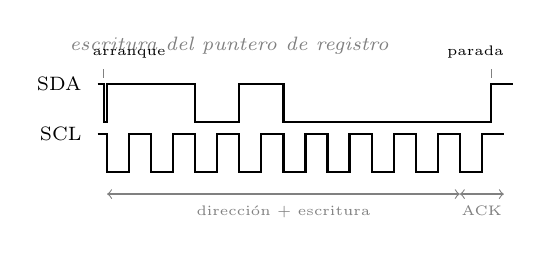
\begin{tikzpicture}[scale=0.8]
        \node[anchor=north west, font=\itshape\scriptsize, gray] at (-0.6,3.4) {escritura del puntero de registro};
        % SDA
        \draw[thick] (0,2.5) -- (0.1,2.5) -- (0.1,1.9) -- (0.15,1.9) -- (0.15,2.5)
            -- (1.55,2.5) -- (1.55,1.9) -- (2.25,1.9) -- (2.25,2.5) -- (2.95,2.5)
            -- (2.95,1.9) -- (6.25,1.9) -- (6.25,2.5) -- (6.6,2.5);
        \node[anchor=east, font=\scriptsize] at (-0.1,2.5) {SDA};
        % SCL
        \draw[thick] (0,1.7) \foreach \i in {0,...,8} {
            -- ({0.15+0.7*\i},1.7) -- ({0.15+0.7*\i},1.1)
            -- ({0.5+0.7*\i},1.1) -- ({0.5+0.7*\i},1.7) } -- (6.45,1.7);
        \node[anchor=east, font=\scriptsize] at (-0.1,1.7) {SCL};
        % condiciones de arranque y parada
        \draw[gray, dashed] (0.1,2.6) -- (0.1,2.75);
        \node[font=\tiny, anchor=south] at (0.5,2.75) {arranque};
        \draw[gray, dashed] (6.25,2.6) -- (6.25,2.75);
        \node[font=\tiny, anchor=south east] at (6.6,2.75) {parada};
        % campos de la trama
        \draw[<->, gray, thin] (0.15,0.75) -- (5.75,0.75);
        \node[gray, font=\tiny, anchor=north] at (2.95,0.72) {dirección + escritura};
        \draw[<->, gray, thin] (5.75,0.75) -- (6.45,0.75);
        \node[gray, font=\tiny, anchor=north] at (6.1,0.72) {ACK};
    \end{tikzpicture}
    \caption[Trama de una transacción I2C de escritura de registro.]{Trama de una transacción I2C completa, en la que el maestro escribe el puntero de registro de un esclavo cuya dirección es \texttt{0x68}. La transmisión comienza con la condición de arranque --SDA baja mientras SCL está alto-- y sigue con ocho pulsos: siete bits de dirección y el bit de escritura. En el noveno pulso el esclavo reconocido responde bajando SDA: es el ACK. A continuación viaja el byte del registro, de nuevo con su ACK, y la transacción termina con la condición de parada. Para \emph{leer} ese registro, el maestro repite el arranque con el bit de lectura en lugar de repetir la dirección entera.}\label{fig:trama_i2c}
\end{marginfigure}

\marginnote{\textbf{Ejemplo de dimensionado:} para el modo rápido (\SI{400}{\kilo\hertz}, $t_{r,max}=\SI{300}{\nano\second}$) con unos \SI{200}{\pico\farad} de bus, la ecuación~\eqref{eq:i2c_pullup} da $R_{p,max} \approx \SI{1.8}{\kilo\ohm}$; en el modo estándar, con $t_{r,max}=\SI{1000}{\nano\second}$, la misma capacidad admite hasta \SI{5.9}{\kilo\ohm}, de ahí que lo habitual sea encontrar \SI{4.7}{\kilo\ohm} en buses lentos y \SI{2}{\kilo\ohm} a \SI{2.2}{\kilo\ohm} en buses rápidos.}

La posibilidad de que el esclavo module el reloj merece una mención aparte: si un dispositivo necesita más tiempo para preparar su respuesta, retiene la línea SCL en nivel bajo y el maestro, que solo puede bajar el reloj, no puede subirlo sin él; la transmisión se alarga tanto como el esclavo necesite. Es el caso único en que un esclavo actúa sobre el reloj y se conoce como \emph{clock stretching}. Al mismo tiempo, si dos maestros comienzan a transmitir a la vez, cada uno escucha el bus mientras habla y, en cuanto lee un nivel distinto del que ha impuesto, sabe que ha perdido el arbitraje: se retira sin haber corrompido nada, porque haber cedido ante un cero ajeno es exactamente lo que el montaje en Y lógico garantiza. El que gana continúa su transacción sin interrupción. Todo ello con una dirección de siete bits --128 combinaciones, de las que 112 son utilizables-- que en la práctica resulta suficiente, porque los integrados de un mismo fabricante rara vez comparten un bus en gran número; cuando no lo es, existe la dirección extendida de diez bits.

\subsection{El Bus SPI}\label{sub:spi}

SPI renuncia a casi todo lo que hace cómodo a I2C para ganar en velocidad y sencillez. Sus cuatro hilos son el reloj (SCLK), el dato del maestro al esclavo (MOSI), el dato del esclavo al maestro (MISO) y la selección del esclavo (CS). Los tres primeros se comparten entre todos los dispositivos y el cuarto es individual: SPI no tiene direcciones, de modo que el maestro elige con quién habla bajando la línea CS de ese esclavo --y solo de ese--. El precio es evidente: un esclavo más exige un pin más, y en un diseño con muchos sensores eso agota antes los pines del microcontrolador que el propio bus.

El resto son ventajas. Los cuatro hilos son de salida activa (push-pull), no de drenador abierto, así que no hacen falta resistencias de polarización y las transiciones son mucho más rápidas: de ahí que SPI funcione a decenas de megahercios mientras el modo típico de I2C en un sensor se queda en \SI{400}{\kilo\hertz}. Además, el bus es \emph{dúplex completo}: en cada pulso de reloj viaja un bit en cada sentido, en lugar de alternar la dirección como en I2C. Para leer los seis bytes de un acelerómetro de tres ejes, esa diferencia es determinante: por I2C, la transacción de la Figura~\ref{fig:trama_i2c} seguida de una lectura de seis bytes ocupa del orden de noventa y dos bits, unos \SI{230}{\micro\second} a \SI{400}{\kilo\hertz}; por SPI bastan cincuenta y seis bits, que a \SI{10}{\mega\hertz} se transmiten en algo menos de \SI{6}{\micro\second}. Y no hay, en cambio, ninguna confirmación por byte: SPI no define ACK ni arbitraje ni control de flujo, y tampoco existe una norma oficial --es un estándar de hecho nacido en Motorola, con variantes entre fabricantes--.

\marginnote{\textbf{La trampa clásica del SPI:} como el reloj puede estar alto o bajo en reposo (polaridad, CPOL) y los datos se pueden muestrear en el flanco de subida o en el de bajada (fase, CPHA), existen cuatro modos de funcionamiento. Si el maestro y el esclavo no coinciden en el modo, la comunicación falla sin dar ningún error de protocolo: los bits llegan, pero con otro significado. Es la primera comprobación ante un sensor SPI que no responde.}

Sin estructura de trama común, cada dispositivo define su propio diálogo: habitualmente un byte de dirección de registro seguido de los datos, o simplemente una secuencia de bytes que el integrado interpreta por posición. El maestro no sabe si el esclavo ha entendido nada, y el esclavo no puede pedir que se le espere; si algo va mal, no lo dirá él, tendrá que detectarlo la aplicación --por ejemplo, comprobando un identificador de dispositivo, muy habitual en los sensores digitales actuales--.

\subsection{Criterios de Elección}\label{sub:criterios_buses}

La elección entre ambos buses rara vez es libre: viene impuesta por lo que ofrece el dispositivo, y muchos de ellos --sobre todo los MEMS-- incorporan las dos interfaces y permiten elegir por un pin o por un registro~\cite{horowitz2015art}. Aun así, conviene tener claro qué gana cada uno, como resume la Tabla~\ref{tab:i2c_vs_spi}. I2C gasta menos pines y ofrece direccionamiento, confirmación y arbitraje; SPI es más rápido, dúplex completo y no necesita resistencias externas. Por eso I2C es el bus natural para leer registros de muchos sensores lentos y memorias pequeñas, mientras que SPI se reserva para lo que exige caudal: convertidores rápidos, memorias de datos, pantallas y tarjetas de memoria.

\begin{table}[ht]
    \centering
    \small
    \setlength{\tabcolsep}{3pt}
    \forceversofloat % la tabla cae en página par (verso); sin forzar, el chequeo de paridad se evalúa antes del salto de página y el caption sale al lado contrario
    \begin{tabularx}{\linewidth}{@{} >{\raggedright\arraybackslash}p{0.24\linewidth} >{\centering\arraybackslash}X >{\centering\arraybackslash}X @{}}
        \toprule
        \textbf{Aspecto} & \textbf{I2C} & \textbf{SPI} \\
        \midrule
        Hilos y pines & Dos (SDA, SCL) & Cuatro, más uno por esclavo (SCLK, MOSI, MISO, CS) \\
        Selección del esclavo & Por dirección de siete bits en la propia trama & Por hardware: una línea CS por esclavo \\
        Sentido de la transmisión & Semidúplex: una dirección cada vez & Dúplex completo: envía y recibe a la vez \\
        Velocidad típica & \SI{100}{\kilo\hertz} a \SI{400}{\kilo\hertz} (hasta \SI{3.4}{\mega\hertz}) & \SI{1}{\mega\hertz} a \SI{10}{\mega\hertz} (hasta decenas de megahercios) \\
        Confirmación por byte & Sí: bit de ACK & No \\
        Control de flujo & Sí: \emph{clock stretching} & No \\
        Varios maestros & Sí, con arbitraje & No \\
        Límite físico & Capacidad de bus $\le$ \SI{400}{\pico\farad}: pocos dispositivos y decenas de centímetros & Integridad de señal de las líneas rápidas; mismo orden de longitud \\
        Uso típico & Registros de sensores, memorias pequeñas, gestión de sistema & Convertidores rápidos, memoria masiva, pantallas \\
        Normalización & Especificación de NXP; derivados SMBus y PMBus & Estándar de hecho, con variantes por fabricante \\
        \bottomrule
    \end{tabularx}
    \caption[Comparación entre los buses I2C y SPI.]{Comparación entre los dos buses de corto alcance. La ventaja de I2C es el cableado y el protocolo --dos hilos compartidos, direccionamiento, reconocimiento y arbitraje--, mientras que la de SPI es el caudal: cuatro hilos sin resistencias externas, dúplex completo y velocidades uno o dos órdenes de magnitud superiores, a cambio de un pin de selección por dispositivo y de ningún mecanismo de confirmación.\protect\label{tab:i2c_vs_spi}}
\end{table}

Los sensores digitales llevan esta idea un paso más allá de lo que sugieren sus registros de configuración. Muchos incorporan un identificador único, guardan en memoria sus propios coeficientes de calibración y publican un mapa de registros con las unidades y el rango de cada magnitud: el dispositivo, en definitiva, sabe describirse a sí mismo. Generalizar esa autodescripción para cualquier sensor, con independencia del fabricante y del bus, es el objetivo de la norma que se estudia en la Sección~\ref{sec:smart_sensors}.

\section{Sensores Inteligentes (\textit{Smart Sensors})}\label{sec:smart_sensors}

Las tres secciones anteriores han seguido el camino de la señal hacia fuera: primero el lazo de corriente que la lleva al puesto de control, después el canal digital que le añade información y, por último, los buses que la mueven dentro del propio equipo. Visto desde el otro extremo, ese recorrido describe una tendencia simétrica: el sensor ha ido absorbiendo la electrónica que antes lo rodeaba. El resultado es el \emph{sensor inteligente} (\textit{smart sensor}), un dispositivo que reúne en un mismo encapsulado el elemento transductor, el acondicionamiento (Capítulo~\ref{cap:opamps}), la conversión analógico-digital (Capítulo~\ref{cap:daq}), un microcontrolador con su memoria y la interfaz de comunicación de la Sección~\ref{sec:i2c_spi}~\cite{frank2013smartsensors}. Este apartado describe qué hay dentro de ese encapsulado (Sección~\ref{sub:anatomia_sensor}), cómo se consigue que cualquier sistema lo reconozca y lo entienda (Sección~\ref{sub:teds}) y qué cambia en la práctica de laboratorio (Sección~\ref{sub:consecuencias_smart}).

\marginnote{\textbf{Qué significa ``inteligente'':} la definición habitual es funcional y deliberadamente amplia: es inteligente el sensor que aporta funciones adicionales a las estrictamente necesarias para representar la magnitud medida. Corregir una no linealidad, compensar la temperatura, vigilarse a sí mismo o describirse para el sistema que lo lee son, todas ellas, funciones ``de más'' que el sensor analógico dejaba en manos del instrumento.}

\subsection{Anatomía de un Sensor Inteligente}\label{sub:anatomia_sensor}

La Figura~\ref{fig:sensor_inteligente} muestra su diagrama de bloques habitual. La cadena analógica de los primeros capítulos aparece íntegra, pero comprimida en unos milímetros: el transductor entrega su señal al acondicionamiento --amplificador y filtro--, y un convertidor A/D la digitaliza. A partir de ahí el trabajo lo hace el microcontrolador: aplicar los coeficientes de calibración, compensar la temperatura, filtrar digitalmente, vigilar el funcionamiento del conjunto, guardar el resultado y atender a la interfaz de comunicación, que puede ser uno de los buses de la Sección~\ref{sec:i2c_spi}, un enlace de un solo hilo o incluso la salida analógica de las Secciones~\ref{sec:lazo_420} y~\ref{sec:hart} con su canal digital superpuesto.

\begin{marginfigure}
    \centering
    \begin{tikzpicture}[scale=0.8, >=Stealth]
        % contorno del encapsulado
        \draw[dashed, gray, thick] (-0.3,2.9) rectangle (5.4,9.4);
        \node[gray, font=\tiny, anchor=north west] at (-0.25,2.85) {encapsulado del sensor};
        % cadena analógica
        \draw[thick] (0.0,8.0) rectangle (3.4,8.8);
        \node[font=\scriptsize] at (1.7,8.4) {Transductor};
        \draw[thick] (0.0,7.0) rectangle (3.4,7.8);
        \node[font=\scriptsize] at (1.7,7.4) {Acondicionamiento};
        \draw[thick] (0.0,6.0) rectangle (3.4,6.8);
        \node[font=\scriptsize] at (1.7,6.4) {ADC};
        % microcontrolador y memoria
        \draw[thick] (0.0,4.6) rectangle (3.4,5.6);
        \node[font=\scriptsize] at (1.7,5.1) {microcontrolador};
        \draw[thick] (4.0,4.6) rectangle (5.2,5.6);
        \node[font=\tiny, align=center] at (4.6,5.1) {memoria\\TEDS};
        \draw[->] (4.0,5.1) -- (3.45,5.1);
        % interfaz
        \draw[thick] (0.0,3.3) rectangle (3.4,4.3);
        \node[font=\tiny, align=center] at (1.7,3.8) {I2C, SPI, 1 hilo\\o lazo 4-20 mA};
        % enlaces
        \foreach \y in {7.95,6.95,5.95,4.25} {
            \draw[->] (1.7,\y) -- (1.7,\y-0.15);
        }
        \draw[->] (1.7,4.6) -- (1.7,4.35);
        % magnitud de entrada y datos de salida
        \draw[->] (1.7,9.9) -- (1.7,8.85) node[midway, right, font=\scriptsize] {$m$};
        \draw[->] (3.4,3.8) -- (5.9,3.8) node[midway, above, font=\tiny] {datos};
    \end{tikzpicture}
    \caption[Diagrama de bloques de un sensor inteligente.]{Diagrama de bloques de un sensor inteligente. Dentro del mismo encapsulado conviven la cadena analógica de los primeros capítulos --transductor, acondicionamiento y convertidor--, un microcontrolador con su memoria de programa y de calibración, y la interfaz de comunicación; esta última puede ser un bus de corto alcance, un enlace de un solo hilo o incluso la salida de lazo de corriente con su canal digital. La memoria guarda tanto el programa de corrección como los coeficientes de calibración y la hoja de datos electrónica del sensor (Sección~\ref{sub:teds}).}\label{fig:sensor_inteligente}
\end{marginfigure}

La linealización es el ejemplo más claro de lo que cambia. En los sensores resistivos del Capítulo~\ref{cap:resistivos} resolvíamos la no linealidad de un termistor con redes analógicas de compensación; en un sensor inteligente el mismo problema se resuelve con aritmética, aplicando al valor digitalizado $x$ el polinomio de corrección que resulta de la calibración,
\begin{equation}\label{eq:linealizacion_digital}
    m = \sum_{i=0}^{n} c_i\,x^i
\end{equation}
cuyos coeficientes $c_i$ viven en la memoria del propio sensor. Lo mismo sucede con la compensación de la deriva térmica, con la corrección del cero y del fondo de escala o con el filtrado: son operaciones que no se desajustan con el tiempo, que no hay que retocar con un destornillador y que pueden repetirse cuantas veces haga falta.

La integración tiene consecuencias que van más allá de la comodidad. En primer lugar, el trayecto analógico se reduce a unos milímetros dentro del encapsulado, de modo que los problemas de ruido, apantallamiento y tierras del Capítulo~\ref{cap:ruido} dejan de pesar: lo que sale del sensor es un número, y un número no se atenúa por el camino ni recoge el zumbido de la red eléctrica. En segundo lugar, el dispositivo puede vigilarse a sí mismo --comprobar que el elemento sensible responde, medir su propia deriva, ejecutar un auto-test-- y comunicar el resultado junto con la medida. Y en tercer lugar, el sistema de adquisición puede leer del sensor lo que antes había que introducir a mano, que es el asunto de la sección siguiente. El precio de todo ello es que el sensor se ha convertido en un pequeño instrumento: depende de su programa, consume energía, tiene una vida comercial más corta que un elemento pasivo y su exactitud sigue acotada por su propia cadena analógica, que no desaparece, sino que se vuelve invisible.

\subsection{La Norma IEEE 1451 y el TEDS}\label{sub:teds}

Que un sensor sea digital resuelve el cableado, pero no resuelve el entendimiento. Para que el sistema de adquisición sepa qué le está llegando --qué magnitud, en qué unidad, con qué sensibilidad y con qué incertidumbre-- hace falta un acuerdo sobre el significado de los datos, y ese acuerdo es el que establece la familia de normas \emph{IEEE 1451}. Su arquitectura separa el procesador que se conecta a la red (\textsc{network capable application processor, ncap}) del módulo que contiene el transductor y su electrónica (\textsc{transducer interface module, tim}); la parte común a toda la familia está en la norma 1451.0, que define las funciones, los comandos y, sobre todo, los formatos de las hojas de datos electrónicas, mientras que los demás miembros cubren el interfaz con microprocesador (1451.2), las redes distribuidas (1451.3), el modo mixto analógico (1451.4), la comunicación inalámbrica (1451.5) y la identificación por radiofrecuencia (1451.7)~\cite{ieee1451_0_2007}.

Esa hoja de datos electrónica --el \emph{teds} (\textsc{transducer electronic data sheet})-- es la pieza central, y su contenido se resume en la Tabla~\ref{tab:teds}. Se trata de una memoria no volátil, habitualmente una EEPROM integrada en el propio sensor o en su conector, que guarda la misma información que la hoja de características en papel, pero en un formato normalizado que el sistema puede leer: la identificación del dispositivo --fabricante, modelo, versión y número de serie, en los 64 bits del bloque básico--, los atributos del transductor, los datos de calibración y un área libre que el usuario puede escribir. La norma define además plantillas para las familias más habituales --acelerómetros, micrófonos, termopares, RTD, galgas, salidas en tensión y en lazo de corriente--, de modo que cada fabricante no inventa su propio formato.

\begin{table}[ht]
    \centering
    \small
    \setlength{\tabcolsep}{3pt}
    \forceversofloat % la tabla cae en página par (verso); sin forzar, el caption sale al lado contrario
    \begin{tabularx}{\linewidth}{@{} >{\raggedright\arraybackslash}p{0.26\linewidth} >{\centering\arraybackslash}X >{\centering\arraybackslash}X @{}}
        \toprule
        \textbf{Bloque} & \textbf{Campos típicos} & \textbf{Para qué sirve} \\
        \midrule
        Identificación (bloque básico) & Fabricante, modelo, versión y número de serie, en 64 bits & Reconocer el sensor y vincularlo a su historial de calibración \\
        Atributos del transductor & Magnitud y tipo, sensibilidad, unidades, rango, polaridad y orientación & Configurar el canal sin introducir datos a mano \\
        Calibración & Fecha y certificado, coeficientes, incertidumbre y curvas o respuestas en frecuencia & Corregir la medida con los datos reales del sensor y no con los nominales del fabricante \\
        Área de usuario & Texto libre: punto de medida, ubicación, notas de mantenimiento & Documentar el canal y su trazabilidad \\
        \bottomrule
    \end{tabularx}
    \caption[Contenido de la hoja de datos electrónica del sensor (TEDS).]{Contenido de la hoja de datos electrónica de un sensor. Los tres primeros bloques describen qué es el dispositivo, cómo hay que interpretar su salida y cómo corregirla; el cuarto queda a disposición del usuario para documentar el canal.\protect\label{tab:teds}}
\end{table}

La parte dedicada al modo mixto (norma 1451.4) merece una atención especial en instrumentación de laboratorio, porque permite que un sensor esencialmente analógico se describa a sí mismo sin renunciar a su salida analógica~\cite{ieee1451_4_2004}. En la clase 1, la memoria del TEDS comparte el mismo hilo que la señal y se lee mediante una breve excursión negativa de la tensión; en la clase 2 ocupa un par propio, compatible con los dispositivos de un solo hilo, lo que simplifica el circuito. El caso típico es el de los acelerómetros piezoeléctricos con electrónica integrada (\textsc{integrated electronics piezo-electric, iepe}) del Capítulo~\ref{cap:generadores}: por el mismo cable coaxial viajan la alimentación de continua --una corriente constante de unos miliamperios-- y la señal de alterna, y junto a ellos un pequeño chip de memoria guarda la sensibilidad del sensor y la fecha de su última calibración, como se esquematiza en la Figura~\ref{fig:teds_mixed}. Al conectar el acelerómetro, el sistema lee primero el TEDS y ya sabe a cuántos milivoltios por unidad de aceleración corresponde su señal; después digitaliza esa señal analógica. La tensión de polarización de continua sirve, además, como el cero vivo del lazo de corriente (Sección~\ref{sec:lazo_420}): un valor anómalo delata un cable abierto o un cortocircuito en la entrada.

\begin{marginfigure}
    \centering
    \begin{tikzpicture}[scale=0.8, >=Stealth]
        % acelerómetro con TEDS
        \draw[thick] (0.0,0.6) rectangle (2.6,3.2);
        \node[font=\scriptsize, align=center] at (1.3,2.85) {Acelerómetro};
        \node[font=\scriptsize, align=center] at (1.3,2.45) {IEPE};
        \draw[thick] (0.3,1.45) rectangle (2.3,2.15);
        \node[font=\tiny, align=center] at (1.3,1.8) {memoria TEDS};
        \draw[thick] (0.3,0.7) rectangle (2.3,1.3);
        \node[font=\tiny, align=center] at (1.3,1.0) {elemento\\piezoeléctrico};
        % cable coaxial
        \draw (2.6,2.0) -- (4.6,2.0);
        \node[font=\tiny, align=center, anchor=south] at (3.6,2.05) {señal y\\alimentación};
        \draw[->] (2.9,1.85) -- (3.3,1.85);
        \draw[<-] (3.9,1.85) -- (4.3,1.85);
        % sistema de adquisición
        \draw[thick] (4.6,0.6) rectangle (6.6,3.2);
        \node[font=\scriptsize, align=center] at (5.6,2.6) {Sistema de};
        \node[font=\scriptsize, align=center] at (5.6,2.2) {adquisición};
        \node[font=\tiny, align=center] at (5.6,1.45) {lee el TEDS\\y digitaliza};
    \end{tikzpicture}
    \caption[Acelerómetro IEPE con TEDS en modo mixto.]{Sensor analógico que se describe a sí mismo: un acelerómetro piezoeléctrico con electrónica integrada (IEPE) y su memoria TEDS. Por el mismo cable coaxial llegan al sensor la alimentación --corriente constante-- y salen la señal de medida y los datos de la memoria. El sistema de adquisición lee primero la hoja de datos electrónica, con la sensibilidad y la fecha de calibración, y solo después convierte la señal analógica.}\label{fig:teds_mixed}
\end{marginfigure}

\subsection{Consecuencias Prácticas}\label{sub:consecuencias_smart}

El efecto inmediato del TEDS es que desaparece la introducción manual de los datos del sensor. En un sistema de muchos canales --una batería de ocho acelerómetros en un ensayo modal, los termopares de una cámara climática-- cada sensor hay que darlo de alta en el software con su sensibilidad, sus unidades y su rango: es un trabajo tedioso y una fuente de error silenciosa, porque introducir la sensibilidad de un sensor en el canal de otro no genera ningún aviso, solo medidas equivocadas. Con TEDS basta conectar: el sistema lee la identificación, la sensibilidad, las unidades y la calibración, y configura el canal por sí mismo. El sensor puede sustituirse por otro del mismo tipo sin tocar el software, y el historial de calibración viaja con el propio dispositivo, con su número de serie y su certificado, lo que simplifica la trazabilidad que exige la metrología del Capítulo~\ref{cap:metrologia}.

A esto se añade la posibilidad de configurar el sensor sin acceder físicamente a él: el rango, la frecuencia de salida de datos, el filtro interno, el auto-test o la puesta a cero se ajustan por software desde el puesto de control. Es la misma dirección hacia la que apuntaban HART (Sección~\ref{sec:hart}) y los buses digitales (Sección~\ref{sec:i2c_spi}): el instrumento deja de tener mandos que girar y pasa a tener parámetros que escribir.

\marginnote{\textbf{Límites que conviene no olvidar:} un sensor inteligente es un pequeño instrumento y hereda sus servidumbres: consume energía, depende de un programa que puede tener errores, envejece antes que un elemento pasivo y su exactitud sigue acotada por su propia cadena analógica y por la cuantización del convertidor (Capítulo~\ref{cap:daq}). La inteligencia no crea exactitud: la traslada y la documenta.}

Con este apartado se cierra el recorrido que abrió el capítulo. El sensor, que en el Capítulo~\ref{cap:resistivos} era una resistencia que había que excitar, leer y corregir, entrega ahora una medida calibrada con sus unidades, su incertidumbre y su identificación; y el sistema de adquisición, protagonista de la cadena de medida en los primeros capítulos, se ha convertido en el cliente de un sensor que sabe describirse a sí mismo.

\section{Resumen}\label{sec:resumen_buses}

En este capítulo se ha completado el último tramo de la cadena de medida --el que separa al sensor acondicionado del sistema de adquisición--, con los medios que la instrumentación industrial y de laboratorio han consensuado para recorrerlo:

\begin{itemize}
    \item \emph{El lazo de corriente 4-20 mA}: transmitir la información como corriente regulada, y no como tensión, hace irrelevantes la resistencia del cable y las perturbaciones inducidas en serie (Figura~\ref{fig:error_cable} y Tabla~\ref{tab:tension_vs_corriente}); el cero vivo en \SI{4}{\milli\ampere} reserva toda la banda inferior para señalar una avería, que nunca se confunde con una medida válida (Figura~\ref{fig:zonas_420}); y el presupuesto de tensión del lazo (Figura~\ref{fig:lazo_420}) es el cálculo que decide cuánta carga y cuánta distancia admite la instalación.
    \item \emph{El protocolo HART}: superpone a esa misma corriente un canal digital por desplazamiento de frecuencia que no altera la medida y que transporta lo que la vía analógica no puede: identificación, calibración, diagnósticos y variables secundarias (Figura~\ref{fig:hart_fsk}). En punto a punto conserva la medida analógica y en multidrop concentra hasta quince instrumentos en un solo par, a costa de repartir entre todos una velocidad de \SI{1200}{\bit\per\second} (Figura~\ref{fig:modos_hart} y Tabla~\ref{tab:modos_hart}).
    \item \emph{Los buses de corto alcance}: dentro del propio equipo, I2C resuelve la conexión con dos hilos compartidos, direcciones de siete bits, reconocimiento por byte y arbitraje entre maestros, sobre una trama cuyas condiciones de arranque y parada reconoce el propio bus (Figuras~\ref{fig:i2c_spi_bus} y~\ref{fig:trama_i2c}); SPI renuncia a todo eso y gasta un hilo de selección por esclavo para ganar en velocidad y en dúplex completo (Tabla~\ref{tab:i2c_vs_spi}).
    \item \emph{Los sensores inteligentes}: el transductor, el acondicionamiento, el convertidor y el microcontrolador conviven ya en el mismo encapsulado (Figura~\ref{fig:sensor_inteligente}), de modo que corregir una no linealidad, compensar la temperatura o ejecutar un auto-test son operaciones aritméticas; su hoja de datos electrónica o TEDS (Tabla~\ref{tab:teds}) hace que el dispositivo se identifique y entregue sus coeficientes de calibración, incluso cuando su salida sigue siendo analógica (Figura~\ref{fig:teds_mixed}).
    \item \emph{De la señal al dato}: los cuatro apartados anteriores son grados de una misma tendencia, el desplazamiento de la inteligencia hacia el sensor. El lazo analógico transportaba un número y nada más; HART le añadió información; los buses digitales le dieron velocidad y direccionamiento; y el TEDS terminó de darle significado. Elegir entre ellos no es buscar el mejor protocolo, sino identificar el eslabón que falta para cada medida (Sección~\ref{sub:criterios_buses}).
\end{itemize}

\marginnote{\textbf{Conclusión:} la señal analógica no desaparece, y el capítulo lo demuestra en cada paso: el lazo de \SI{4}{\milli\ampere} a \SI{20}{\milli\ampere} sigue llevando la medida mientras el canal digital lleva la información, y un sensor inteligente puede seguir teniendo salida analógica. La lección no es que lo digital sustituya a lo analógico, sino que ambos conviven --analógico para la medida continua, digital para su contexto-- y que elegir el eslabón adecuado en cada caso es una decisión de ingeniería, no de moda.}
